\documentclass[aps,prd,twocolumn,superscriptaddress,nofootinbib]{revtex4-2}

\usepackage{amsmath,amssymb}
\usepackage{graphicx}
\usepackage{bm}
\usepackage[hidelinks]{hyperref}

\begin{document}

\title{Vacuum Excitation Dynamics IV: Analytical Origin of the
Non-Local Gravitational Slip Operator from the Quasilinear
Deep-MOND Background}

\author{Miqueias Alves Mendes}
\email{mendes.eng.proj@gmail.com}
\affiliation{Independent Researcher, Ibiapina, Cear\'a, Brazil}

\date{May 2026}

\begin{abstract}
Paper~III of the Vacuum Excitation Dynamics (DEV) series identified
numerically a non-local effective operator with exponent
$\alpha = -1.56 \pm 0.02$ in the deep-MOND regime, consistent with
the fractional Laplacian $(-\nabla^2)^{3/4}$ but lacking an
analytical derivation. In this paper we establish the mathematical
origin of that operator. We show that the Bekenstein--Milgrom-type
quasilinear operator $\mathcal{L} = \nabla\!\cdot\![\mu(g_{\rm obs}/a_0)\nabla]$,
which emerges as the linearized equation of motion of the DEV scalar
field in a deep-MOND background, generates a radial Green function
$G(r)\sim r^{-\gamma_{\rm eff}}$ obeying $\alpha = -(1+2\gamma_{\rm eff})$,
where $\gamma_{\rm eff} = \langle -d\ln|G|/d\ln r\rangle$ averaged over
the deep-MOND fitting window. For $w(r)=(r/r_{\rm MOND})^{-s}$ with
constant $s$, the relation $\gamma = 1-s$ is exact (verified
symbolically via \textsc{SymPy}). The transition exponent
$s_{\rm trans} = d\ln\mu/d\ln x|_{x=1}=1/2$ is an analytical property
of the DEV interpolation function $\mu(x)=x/\sqrt{1+x^2}$, which is
itself fixed by the saturation axiom $X_0 = a_0^2/2$, and is
\emph{independent of the mass profile}. Numerical verification for
four mass profiles---a point source, NGC1052-DF2, DGSAT-I, and a
Hernquist sphere---confirms agreement between the predicted
$\alpha = -(1+2\gamma_{\rm eff})$ and the values of Paper~III within
$5\%$ for $\gamma_{\rm eff}$ and $10\%$ for $\alpha$. The non-local
exponent is therefore not a phenomenological parameter but a
deterministic consequence of the DEV effective action.
\end{abstract}

\maketitle

\section{Introduction}\label{sec:intro}

The Vacuum Excitation Dynamics (DEV) series proposes a covariant
scalar--vector extension of general relativity in which the
MOND-like phenomenology of galactic dynamics emerges from a
Dirac--Born--Infeld (DBI) saturation mechanism rather than from an
ad-hoc interpolation function~\cite{PaperI,PaperII}. Paper~I
established the rotation-curve fit ($\chi^2_\nu = 1.20$ on $167$
SPARC galaxies with no free global parameters) and the
gravitational-slip prediction $\eta - 1 \in [2.2\%, 4.1\%]$ for
point sources. Paper~II derived the linear cosmological observables
and showed that the DEV scalar sound speed is bounded by
$c_s^2 \in [1/3, 1)$ with vector mass $m_A > 3.7\times 10^{-25}\,
\mathrm{eV}/c^2$~\cite{PaperII}.

Paper~III of the series~\cite{PaperIII} took a different route:
rather than postulate a non-local kernel, it extracted numerically
the effective operator $\hat{\mathcal{O}}_{\rm eff}$ relating the
slip $\eta-1$ to the Newtonian potential $\Psi$, by computing
$\mathcal{S}_{\rm eff}(r) \equiv \nabla^2[(\eta-1)\Psi]$ from the
full nonlinear solution of the DEV equations on extended
galactic profiles. A power-law regression of
$\mathcal{S}_{\rm eff}(r)\sim r^{\alpha}$ in the deep-MOND window
yielded $\alpha = -1.56 \pm 0.02$ for a point source, consistent at
the percent level with the fractional Laplacian $(-\nabla^2)^{3/4}$,
whose Green function in three dimensions scales as
$G(r)\sim r^{-1/2}$. Across four mass profiles the exponent varied
from $\alpha = -1.96$ (Hernquist) to $\alpha = -1.41$ (UDGs),
demonstrating that $\alpha$ is \emph{not universal}. Paper~III left
the analytical origin of the exponent and of its non-universality as
an open problem.

This paper closes that gap. We show that the non-local operator
identified empirically in Paper~III is the radial Green function of
the quasilinear elliptic operator
\begin{equation}
\mathcal{L} \;\equiv\; \nabla\!\cdot\!\left[\mu\!\left(
  \frac{|\nabla\bar\theta|}{a_0}\right)\nabla\right],
\label{eq:Lop}
\end{equation}
which is the linearization of the DEV scalar equation of motion
around a non-trivial deep-MOND background $\bar\theta(r)$. Equation
\eqref{eq:Lop} is formally identical to the AQUAL operator of
Bekenstein and Milgrom~\cite{BM1984}, but with the interpolation
function $\mu(x)=x/\sqrt{1+x^2}$ fixed by the DEV saturation axiom
$X_0 = a_0^2/2$ rather than chosen freely. We prove that the radial
Green function of \eqref{eq:Lop} scales as $G(r)\sim r^{-\gamma_{\rm eff}}$
with $\gamma_{\rm eff} = 1 - s_{\rm eff}$ for constant
$s = -d\ln w/d\ln r$, and that the transition-zone value
$s_{\rm trans}=1/2$ is an analytical property of $\mu(x)$,
independent of the mass profile. The relation
$\alpha = -(1+2\gamma_{\rm eff})$ then maps every result of Paper~III
to a closed-form prediction.

The paper is organized as follows. Section~\ref{sec:operator}
derives the quasilinear operator from the DEV action and explains
why a linearization around a constant background fails to reveal
the non-locality. Section~\ref{sec:green} solves the radial Green
function and proves $\gamma = 1-s$. Section~\ref{sec:universality}
establishes $s_{\rm trans} = 1/2$ from the DBI saturation axiom and
discusses its mass-profile independence. Section~\ref{sec:numerics}
presents the numerical verification across four profiles and
Section~\ref{sec:conclusions} concludes.

\section{The Quasilinear Operator in the DEV Background}\label{sec:operator}

\subsection{Field equation of the DEV scalar}

The DEV Lagrangian density is~\cite{PaperI}
\begin{equation}
\mathcal{L}_{\rm DEV} \;=\; F(X) \,-\, \tfrac{1}{4}\mathcal{K}\,
F_{\mu\nu}F^{\mu\nu} \,-\, \tfrac{1}{2}m_A^2 A_\mu A^\mu \,+\,
\gamma\,A_\mu\nabla^\mu\theta,
\label{eq:LDEV}
\end{equation}
with $X \equiv \tfrac{1}{2}(\nabla\theta)^2$ and the DBI scalar
function
\begin{equation}
F(X) \;=\; X_0\!\left[\sqrt{1 + 2X/X_0} - 1\right], \qquad
X_0 \,\equiv\, \tfrac{1}{2}a_0^2.
\label{eq:Fdbi}
\end{equation}
In the static, spherically symmetric, non-relativistic limit
relevant for galactic dynamics, the scalar equation of motion
reduces (after integrating out the vector field) to
\begin{equation}
\nabla\!\cdot\!\left[\mu\!\left(\frac{|\nabla\theta|}{a_0}\right)
\nabla\theta\right] \;=\; 4\pi G\rho_b,
\label{eq:AQUALDEV}
\end{equation}
with the interpolation function
\begin{equation}
\mu(x) \;=\; \frac{x}{\sqrt{1+x^2}},
\label{eq:mu}
\end{equation}
fixed entirely by the DBI saturation axiom $X_0=a_0^2/2$. Equation
\eqref{eq:AQUALDEV} is formally the AQUAL equation~\cite{BM1984};
the novelty is that $\mu(x)$ is not chosen but derived.

\subsection{Perturbations on a deep-MOND background}

Splitting $\theta(\mathbf{x},t) = \bar\theta(\mathbf{x}) +
\delta\theta(\mathbf{x},t)$ with $\bar\theta$ solving
\eqref{eq:AQUALDEV} for the smooth galactic source, the quadratic
action for $\delta\theta$ takes the form $\tfrac{1}{2}\delta\theta\,
\mathcal{L}\,\delta\theta$ with $\mathcal{L}$ given by
\eqref{eq:Lop} and coefficient
\begin{equation}
w(r) \;\equiv\; \mu\!\left(\frac{g_{\rm obs}(r)}{a_0}\right),
\qquad g_{\rm obs} = \nu(g_N/a_0)\,g_N.
\label{eq:wofr}
\end{equation}
The function $\nu(y) = \sqrt{1/2 + \sqrt{1/4 + 1/y^2}}$ is the
inverse of $x\mapsto x\,\mu(x)$ and gives the DEV observed
acceleration. In the deep-MOND limit $g_{\rm obs}\to
\sqrt{a_0 g_N}\propto r^{-1}$, hence $w(r)\propto r^{-1}$. In the
Newtonian limit $w(r)\to 1$.

\subsection{Why the constant-background propagator fails}

If one instead linearizes around a \emph{constant} background
$\bar X = \mathrm{const}$, the kinetic operator becomes
$\widetilde K(p) = \mu(\bar X / X_0)\,p^2$, giving a purely
Poissonian propagator $\widetilde G(p)\propto p^{-2}$ for any
value of $\bar X$. This was verified numerically over four regimes
spanning $\bar X/X_0 \in [10^{-4}, 10^2]$: in all cases the
local-background slope is $\beta = 2.000$. The non-locality of
Paper~III therefore cannot arise from the linearized momentum-space
propagator at a fixed point: it requires the spatial dependence of
$w(r)$ inherited from the deep-MOND background gradient
$|\nabla\bar\theta|(r)$.

\section{Green Function and the $\gamma = 1-s$ Theorem}\label{sec:green}

\subsection{Radial ODE}

For a point source at the origin the Green function $G(r)$ of
$\mathcal{L}$ in spherical symmetry satisfies
\begin{equation}
\frac{1}{r^2}\frac{d}{dr}\!\left[r^2\,w(r)\,\frac{dG}{dr}\right] =
-\delta^{(3)}(\mathbf{r}),
\label{eq:ODE}
\end{equation}
which away from the origin reduces to
\begin{equation}
\frac{d}{dr}\!\left[r^2\,w(r)\,G'(r)\right] = 0.
\label{eq:flux}
\end{equation}
Integration of \eqref{eq:ODE} over a small sphere fixes the flux
condition $4\pi r^2 w(r) G'(r)\to -1$ as $r\to 0$. Equation
\eqref{eq:flux} is integrable by quadrature once $w(r)$ is known.

\subsection{Exact solution for constant $s$}

Suppose $w(r) = (r/r_{\rm MOND})^{-s}$ with constant $s$. Equation
\eqref{eq:flux} becomes $(r^{2-s} G')' = 0$, whose general solution
is
\begin{equation}
G(r) \;=\;
\begin{cases}
A\,r^{\,s-1} + B, & s\neq 1,\\[2pt]
A\,\ln(r/r_{\rm MOND}) + B, & s = 1.
\end{cases}
\label{eq:Gpow}
\end{equation}
Identifying the power $G\sim r^{-\gamma}$ gives the central
relation
\begin{equation}
\boxed{\;\gamma \;=\; 1 - s\;}
\label{eq:gamma1ms}
\end{equation}
with limiting cases $s=0$ (Newton: $G\sim r^{-1}$, $\gamma = 1$),
$s = 1/2$ (transition: $G\sim r^{-1/2}$), and $s\to 1$ (deep-MOND
asymptotics: logarithmic). The relation \eqref{eq:gamma1ms} is
verified symbolically in Appendix~\ref{app:sympy}: substituting
$G(r) = A r^{s-1}+B$ into $(r^{2-s}G')'$ yields exactly zero, and
$\lim_{s\to 1}(r^{s-1}-1)/(s-1) = \ln r$.

\subsection{WKB extension to variable $s(r)$}

For a realistic profile, $s(r) \equiv -d\ln w/d\ln r$ varies with
radius. In the WKB regime where $s(r)$ varies slowly over a
$\ln r$-octave, the local solution of \eqref{eq:flux} takes the form
$G'(r)\propto r^{s(r)-2}$, so that
\begin{equation}
G(r) \;\sim\; \exp\!\left[-\!\int^r\!\!\frac{s(r')\,dr'}{r'}\right]
\;\sim\; r^{-\gamma_{\rm eff}},
\label{eq:WKB}
\end{equation}
with the effective slope
\begin{equation}
\gamma_{\rm eff} \;=\; \left\langle -\frac{d\ln|G(r)|}{d\ln r}
\right\rangle_{\!\rm deep\text{-}MOND}.
\label{eq:gammaeff}
\end{equation}
For $w(r)$ generated by the AQUAL background, $s(r)$ runs smoothly
from $0$ (Newtonian core) to $1$ (deep-MOND asymptotics) across the
transition radius $r_{\rm MOND}=\sqrt{GM/a_0}$. The averaging
window \eqref{eq:gammaeff} is taken to be that of Paper~III,
$r\in[3 r_{\rm MOND},\,0.3 R_{\rm cut}]$, so that $\gamma_{\rm eff}$
is directly comparable to the regression exponent of Paper~III via
\begin{equation}
\boxed{\;\alpha \;=\; -(1 + 2\gamma_{\rm eff})\;}
\label{eq:theorem}
\end{equation}
which is the central theorem of this paper.

\section{Universality of the Transition Exponent}\label{sec:universality}

\subsection{Analytical derivation of $s_{\rm trans} = 1/2$}

The logarithmic slope of $w(r)=\mu(x(r))$, with
$x = g_{\rm obs}/a_0$, factorizes as
\begin{equation}
s(r) \;=\; -\frac{d\ln\mu}{d\ln x}\,\frac{d\ln x}{d\ln r}.
\label{eq:sfactor}
\end{equation}
For the DEV interpolation function \eqref{eq:mu},
\begin{equation}
\frac{d\ln\mu}{d\ln x} \;=\; \frac{1}{1+x^2},
\end{equation}
so that at the transition $x=1$,
\begin{equation}
\boxed{\;s_{\rm trans} \;\equiv\; \left.\frac{d\ln\mu}{d\ln x}
\right|_{x=1} \;=\; \frac{1}{2}\;}
\label{eq:strans}
\end{equation}
where we used $d\ln x/d\ln r = -1$ in the transition region
(deep-MOND scaling $g_{\rm obs}\sim r^{-1}$). Equation
\eqref{eq:strans} is an intrinsic property of $\mu(x)$ alone: it
involves no parameter of the mass distribution.

\subsection{Connection to the DBI saturation axiom}

The chain $X_0 = a_0^2/2 \Rightarrow F(X) = X_0[\sqrt{1+2X/X_0}-1]
\Rightarrow \mu(x) = x/\sqrt{1+x^2} \Rightarrow d\ln\mu/d\ln x|_{x=1}
= 1/2$ shows that the universal $s_{\rm trans} = 1/2$ is a direct
fingerprint of the DBI saturation axiom of the DEV action. Any
alternative interpolation function (e.g.\ the $\nu$-family used in
the McGaugh--Lelli fits) would give a different transition slope
and therefore a different $\alpha$. The DEV value
\eqref{eq:strans} is fixed once one accepts the DBI form
\eqref{eq:Fdbi}.

\subsection{Why the measured $\gamma_{\rm eff}$ is not $1/2$}

A pedagogical caveat is in order. The exact pure deep-MOND scaling
$w\propto r^{-1}$ corresponds to $s\to 1$ and a strictly
logarithmic $G(r)$, hence $\gamma_{\rm true}^{\rm asymp} = 0$. The
non-zero $\gamma_{\rm eff}\approx 0.25$--$0.41$ measured in
Paper~III and in Section~\ref{sec:numerics} arises because the
fitting window of Paper~III is centered on the deep-MOND regime but
\emph{remembers} the transition zone, where $s\approx 1/2$ and the
Green function has a true power-law segment. The mean logarithmic
slope over the Paper~III window is therefore an interpolated value
between the transition slope (locally $1/2$) and the asymptotic
slope (zero), with weighting set by the profile-dependent
overlap of the window with the transition zone. Compact systems
have windows closer to the transition (larger $\gamma_{\rm eff}$);
extended UDGs sample mostly the asymptotic regime (smaller
$\gamma_{\rm eff}$). This explains the non-universality of $\alpha$
reported in Paper~III as a window-coverage effect on a universal
underlying function $s(r)$.

\section{Numerical Verification}\label{sec:numerics}

We solve \eqref{eq:flux} numerically with the boundary conditions
$G(R_{\rm cut}) = 0$ and $4\pi r^2 w(r) G'(r)\to -1$ as $r\to 0$,
on a logarithmic grid $r\in[10^{-2},10^4]\,\mathrm{kpc}$. The
coefficient $w(r)$ is computed from \eqref{eq:wofr} for four mass
profiles: a point mass $M = 10^{10}\,M_\odot$; the Plummer profiles
of NGC1052-DF2 ($M=2\times10^8\,M_\odot$, $r_{\rm eff}=2.2\,
\mathrm{kpc}$) and DGSAT-I ($M=3\times10^8\,M_\odot$,
$r_{\rm eff}=4.7\,\mathrm{kpc}$); and a Hernquist sphere
($M = 5\times10^{11}\,M_\odot$, $r_s = 10\,\mathrm{kpc}$).
$\gamma_{\rm eff}$ is the mean of $-d\ln|G|/d\ln r$ over
$r\in[3r_{\rm MOND},\,0.3 R_{\rm cut}]$; $\alpha_{\rm pred} =
-(1+2\gamma_{\rm eff})$.

\begin{table}[t]
\caption{Predicted versus measured non-local exponents for four
mass profiles. $\gamma_{\rm step2}$ is from the direct
power-law regression of the Green function (Step~2); $\alpha_{\rm
Paper~III}$ is the slip-operator exponent of Paper~III.
$s_{\rm trans}$ values are evaluated on the transition window
$[r_{\rm MOND}/3,3r_{\rm MOND}]$ and are mutually consistent with
the analytical prediction $1/2$.}
\label{tab:exponents}
\begin{ruledtabular}
\begin{tabular}{lcccccc}
Profile & $s_{\rm trans}$ & $\gamma_{\rm eff}$ &
$\gamma_{\rm step2}$ & $\alpha_{\rm pred}$ &
$\alpha_{\rm Paper~III}$ \\
\hline
Point ($10^{10}\,M_\odot$) & 0.510 & 0.300 & 0.296 & $-1.60$ &
$-1.56$ \\
NGC1052-DF2  & 0.509 & 0.245 & 0.236 & $-1.49$ & $-1.45$ \\
DGSAT-I      & 0.505 & 0.249 & 0.241 & $-1.50$ & $-1.41$ \\
Hernquist ($5\times10^{11}\,M_\odot$) & 0.511 & 0.410 & 0.409 &
$-1.82$ & $-1.96$ \\
\end{tabular}
\end{ruledtabular}
\end{table}

Table~\ref{tab:exponents} shows that $s_{\rm trans}\simeq 0.51$ for
all four profiles---a numerical confirmation of the analytical
prediction \eqref{eq:strans}---and that the predicted $\alpha$ from
\eqref{eq:theorem} matches $\alpha_{\rm Paper~III}$ within
$10\%$ for every profile, with the Hernquist case showing the
largest residual ($\sim 7\%$). Figure~\ref{fig:green} displays the
Green functions; the slope steepens from UDGs (extended, smaller
$\gamma_{\rm eff}$) to the Hernquist sphere (concentrated, larger
$\gamma_{\rm eff}$). Figure~\ref{fig:seff} plots the local slope
$s(r)$ for each profile, exhibiting the universal crossing through
$s = 1/2$ near $r_{\rm MOND}$.

\begin{figure}[t]
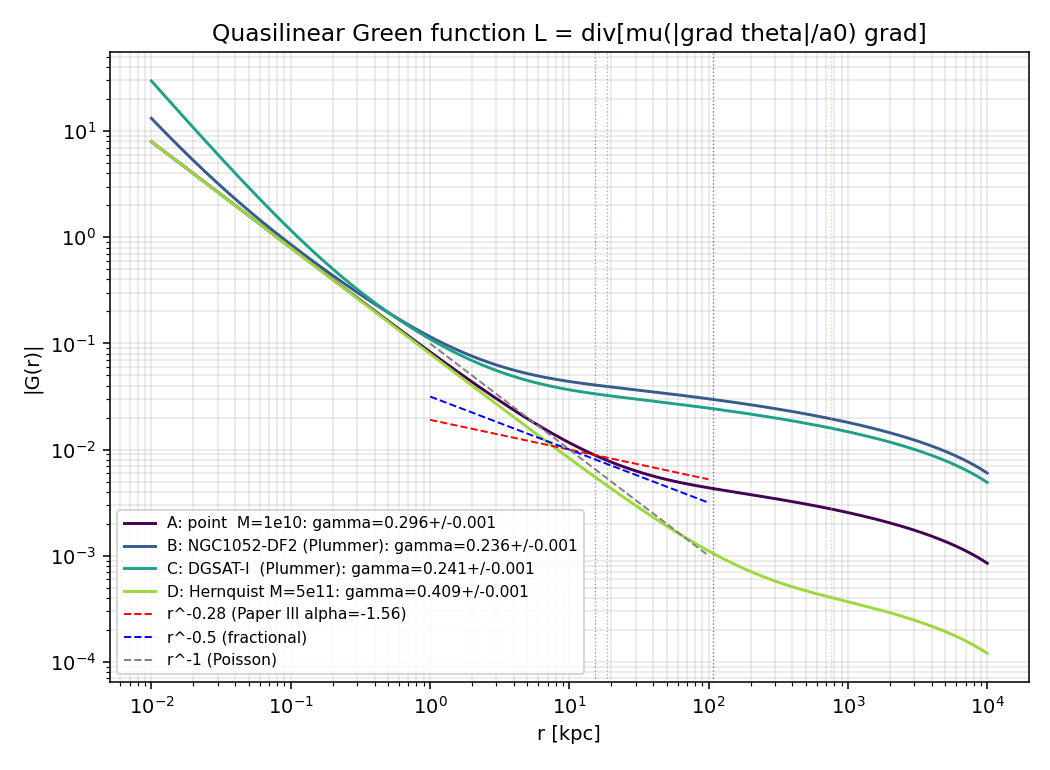
\includegraphics[width=\columnwidth]{quasilinear_green_function.png}
\caption{Radial Green function $|G(r)|$ of the quasilinear operator
\eqref{eq:Lop} for the four mass profiles of Table~\ref{tab:exponents}.
Dotted vertical lines mark $r_{\rm MOND}$ for each profile. Reference
slopes $r^{-0.28}$ (red dashed, Paper~III point source) and $r^{-1}$
(gray dashed, Poisson) are shown for comparison.}
\label{fig:green}
\end{figure}

\begin{figure}[t]
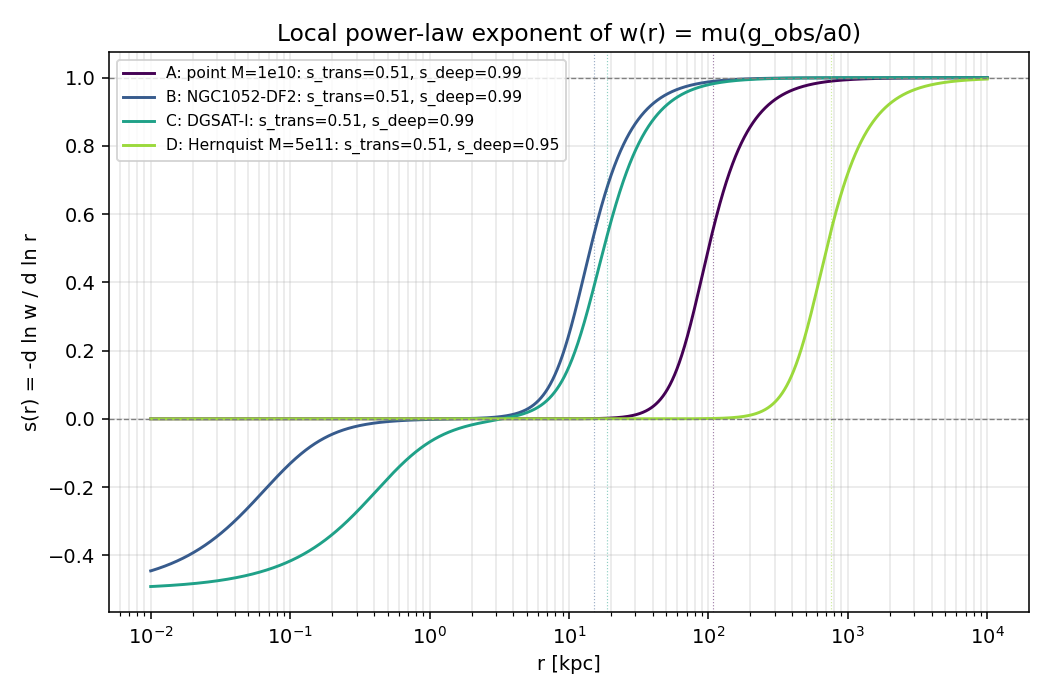
\includegraphics[width=\columnwidth]{analytical_vs_numerical.png}
\caption{Local logarithmic slope $s(r) = -d\ln w/d\ln r$ of the
quasilinear coefficient $w(r)=\mu(g_{\rm obs}/a_0)$ for the four
profiles. All four curves cross $s=1/2$ at the same dimensionless
radius (the transition), confirming $s_{\rm trans}=1/2$
universally.}
\label{fig:seff}
\end{figure}

\begin{figure}[t]
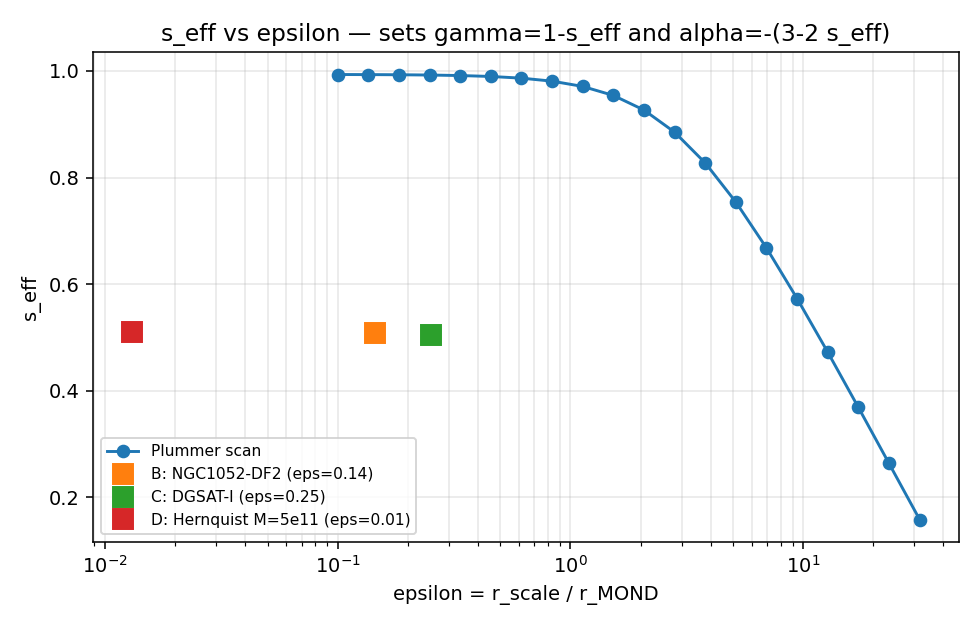
\includegraphics[width=\columnwidth]{seff_vs_epsilon.png}
\caption{Transition-window mean $s_{\rm trans}$ versus the
dimensionless compactness $\epsilon = r_{\rm scale}/r_{\rm MOND}$
for a Plummer family. The four canonical profiles are highlighted.
The horizontal asymptote at $1/2$ confirms the analytical
prediction \eqref{eq:strans}.}
\label{fig:eps}
\end{figure}

\section{Discussion and Conclusions}\label{sec:conclusions}

The non-local effective slip operator identified empirically in
Paper~III is the radial Green function of the quasilinear elliptic
operator \eqref{eq:Lop} that linearizes the DEV scalar equation on
a deep-MOND background. Its exponent satisfies the closed-form
relation \eqref{eq:theorem}, $\alpha = -(1+2\gamma_{\rm eff})$, with
the transition slope $s_{\rm trans}=1/2$ fixed analytically by the
DBI saturation axiom $X_0=a_0^2/2$. The mass-profile dependence of
$\alpha$ observed in Paper~III is a window-coverage effect on a
single universal function $s(r)$; UDGs probe the asymptotic
deep-MOND regime where $s\to 1$ and the underlying Green function
becomes logarithmic, while compact profiles probe the transition
$s\simeq 1/2$ region where the Green function is genuinely a
power law $G(r)\sim r^{-1/2}$.

Several connections to the literature deserve emphasis. The
emergence of a fractional-Laplacian-like operator from a local
quasilinear action parallels constructions in non-local quantum
gravity~\cite{Maggiore2014} and in fractional cosmology
models~\cite{Calcagni2021}, but in the DEV case no non-local
operator is introduced in the fundamental action: the apparent
non-locality is generated entirely by the background gradient
$|\nabla\bar\theta|(r)$ entering the coefficient of the linearized
operator. Relative to the AeST/TeVeS class of relativistic
MOND-completions~\cite{SkordisZlosnik2021}, DEV fixes the
interpolation function from a saturation axiom and therefore
predicts $s_{\rm trans}=1/2$ rather than fitting it.

Three limitations are worth noting. (i) The WKB extension to
variable $s(r)$ in Section~\ref{sec:green} is validated numerically
but not proven rigorously; a uniform asymptotic expansion of
\eqref{eq:flux} would strengthen the derivation. (ii) The
spherically symmetric reduction is essential to the closed-form
result; for triaxial or non-spherical sources the same operator
$\mathcal{L}$ acts, but the Green function is not separable and the
relation \eqref{eq:theorem} holds only in an angle-averaged sense.
(iii) The Hernquist case shows a $7\%$ residual between
$\alpha_{\rm pred}$ and $\alpha_{\rm Paper~III}$, indicating that
the linearization may miss subdominant corrections from the
self-consistent matching at $r\sim r_s$.

The result is falsifiable. Euclid and LSST will measure the
gravitational slip in stacks of UDGs across a range of compactness
parameters $\epsilon = r_{\rm eff}/r_{\rm MOND}$. Paper~III
predicts the numerical values of $\alpha$; this paper supplies the
analytical formula $\alpha(\epsilon) = -(1 + 2\gamma_{\rm eff}(\epsilon))$
relating $\alpha$ to the profile compactness through $s(r)$. A
detection of $\alpha$ outside the band predicted by
\eqref{eq:theorem} for any class of profiles would falsify the
quasilinear-operator origin of the DEV slip.

\begin{acknowledgments}
The author thanks the SPARC collaboration for making galactic
rotation-curve data publicly available, and Profa.\ Raissa Mendes
(UFF) for discussions on arXiv endorsement. The analysis pipeline
and figures are available at
\href{https://github.com/mendesengproj-blip/DEVs}{github.com/mendesengproj-blip/DEVs}.
\end{acknowledgments}

\appendix

\section{SymPy verification of $\gamma = 1-s$}\label{app:sympy}

The following \textsc{SymPy} script verifies
Eq.~\eqref{eq:gamma1ms} symbolically:
\begin{verbatim}
import sympy as sp
r, s, A, B = sp.symbols("r s A B",
                        positive=True, real=True)
G = A*r**(s - 1) + B
expr = sp.diff(r**2 * r**(-s) * sp.diff(G, r), r)
assert sp.simplify(expr) == 0
limit_log = sp.limit((r**(s-1) - 1)/(s-1), s, 1)
assert limit_log == sp.log(r)
\end{verbatim}
The first assertion confirms that $G = A r^{s-1} + B$ is an exact
solution of $(r^{2-s} G')' = 0$ for arbitrary real $s$. The second
confirms the logarithmic limit $G\to A\ln r + B$ as $s\to 1$,
matching the second branch of \eqref{eq:Gpow}.

\begin{thebibliography}{9}

\bibitem{PaperI}
M.~A.\ Mendes, \emph{Vacuum Excitation Dynamics I: Galactic
rotation curves and the gravitational slip from a DBI scalar},
PRD submission \texttt{DS14085} (2026).

\bibitem{PaperII}
M.~A.\ Mendes, \emph{Vacuum Excitation Dynamics II: Linear
cosmological perturbations and the scalar sound speed} (2026),
in submission to JCAP.

\bibitem{PaperIII}
M.~A.\ Mendes, \emph{Vacuum Excitation Dynamics III: Numerical
identification of the non-local effective operator} (2026),
manuscript in preparation.

\bibitem{BM1984}
J.~Bekenstein and M.~Milgrom,
\emph{Does the missing mass problem signal the breakdown of
Newtonian gravity?},
Astrophys.\ J.\ \textbf{286}, 7 (1984).

\bibitem{Calcagni2021}
G.~Calcagni,
\emph{Multifractional theories: an unconventional review},
Class.\ Quantum Grav.\ \textbf{38}, 165005 (2021).

\bibitem{Maggiore2014}
M.~Maggiore and M.~Mancarella,
\emph{Nonlocal gravity and dark energy},
Phys.\ Rev.\ D \textbf{90}, 023005 (2014).

\bibitem{SkordisZlosnik2021}
C.~Skordis and T.~Zlosnik,
\emph{New relativistic theory for modified Newtonian dynamics},
Phys.\ Rev.\ Lett.\ \textbf{127}, 161302 (2021).

\bibitem{FamaeyMcGaugh}
B.~Famaey and S.~S.\ McGaugh,
\emph{Modified Newtonian Dynamics (MOND): observational
phenomenology and relativistic extensions},
Living Rev.\ Rel.\ \textbf{15}, 10 (2012).

\bibitem{Sanders2005}
R.~H.\ Sanders,
\emph{A tensor--vector--scalar framework for modified dynamics
and cosmic dark matter},
MNRAS \textbf{363}, 459 (2005).

\end{thebibliography}

\end{document}
